\documentclass{article}

\usepackage{tikz}
\pgfdeclarelayer{bg}
\pgfsetlayers{bg,main}

\begin{document}

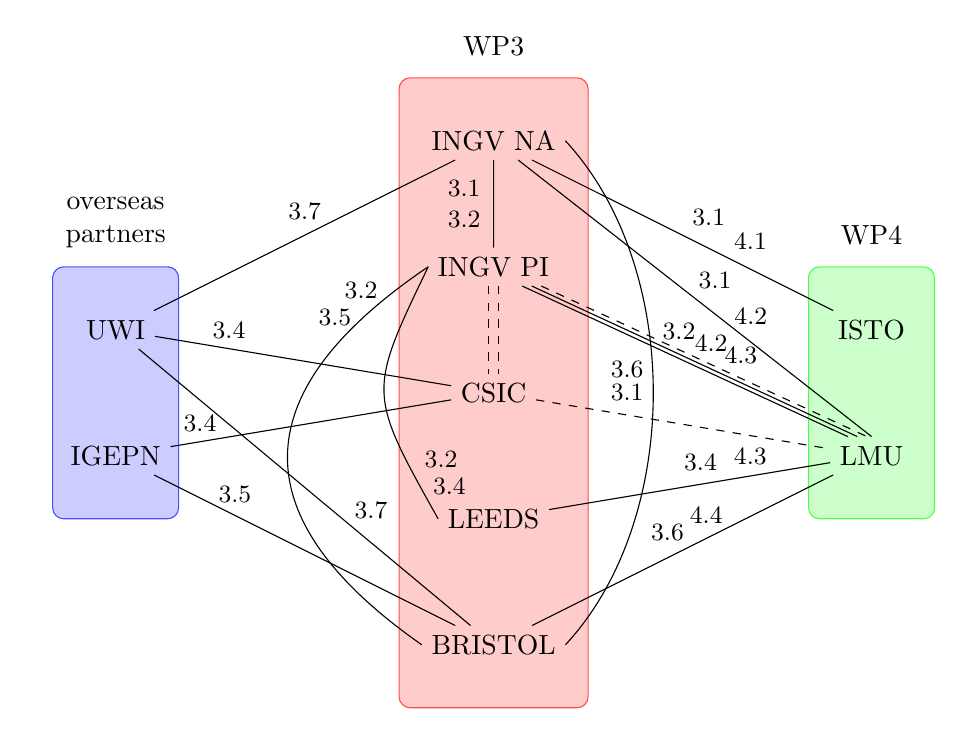
\begin{tikzpicture}
  [scale=.8,auto=left,every node/.style={rectangle}]
  \node (n1) at (7,9)  {INGV NA};
  \node (n2) at (7,7)  {INGV PI};
  \node (n3) at (7,5)  {CSIC};
  \node (n4) at (7,3)  {LEEDS};
  \node (n5) at (7,1)  {BRISTOL};
  \node (n6) at (1,4)  {IGEPN};
  \node (n7) at (1,6)  {UWI};
  \node (n8) at (13,6)  {ISTO};
  \node (n9) at (13,4)  {LMU};

\draw (n1) -- node[left,text width=0.5cm,text centered,font=\small]
{3.1 3.2} (n2);
\draw (n1) -- node[font=\small] {3.1}
node[xshift=3.5ex,yshift=-2ex,font=\small] {4.1} (n8);
\draw (n1) -- node[yshift=0.5ex,above,font=\small] {3.7} (n7);
\draw(n3) -- node[near end,above,font=\small] {3.4} (n7);
\draw(n3) -- node[xshift=-2pt,very near end,above,font=\small] {3.4} (n6);
\draw(n4) -- node[xshift=-12pt,yshift=-2pt,near end,font=\small] {3.4}
node[xshift=6pt,near end,font=\small] {4.3}(n9);
\draw(n5) -- node[xshift=4pt,font=\small] {3.6}
node[xshift=18pt,yshift=6pt,font=\small] {4.4} (n9);
\draw(n5) -- node[xshift=2pt,above,near end,font=\small] {3.5} (n6);
\draw(n5) -- node[xshift=-6pt,yshift=10pt,above, near start,font=\small] {3.7} (n7);
\draw (n1) -- node[xshift=-0.5ex,font=\small] {3.1}
node[xshift=2.5ex,yshift=-3ex,font=\small] {4.2}(n9.north);
\draw (n2.west) .. controls (5,5) .. node[very near end,font=\small] {3.2}
node[very near end,xshift=0.7ex,yshift=-2.3ex,font=\small] {3.4} (n4.west);
\draw (n2.west) .. controls (3,5) and (3,3) .. node[left,very near
start,xshift=1.7ex,yshift=2ex,font=\small] {3.2} node[left,very near
start,xshift=-0.5ex,yshift=-0.3ex,font=\small] {3.5} (n5.west);
\draw (n1.east) .. controls (10,7) and (10,3) .. node[left,font=\small]
{3.1} node[left,yshift=2ex,font=\small] {3.6} (n5.east);

\begin{scope}[style=dashed]
  \draw ([xshift=5ex]n2.south) -- ([xshift=-0.5ex]n9.north);
  \draw (n3) -- (n9);
\end{scope}
\draw[dashed] ([xshift=0.5ex]n2.south) -- ([xshift=0.5ex]n3.north);
\draw[dashed] ([xshift=-0.5ex]n2.south) -- ([xshift=-0.5ex]n3.north);
\draw ([xshift=4ex]n2.south) -- node[xshift=-3.5ex,yshift=1ex,font=\small] {3.2}
([xshift=-1.5ex]n9.north);

\draw ([xshift=3ex]n2.south) --
node[font=\small] {4.2} node[xshift=2.5ex,yshift=-1ex,font=\small]
{4.3} ([xshift=-2.5ex]n9.north);

\begin{pgfonlayer}{bg}
  \filldraw[fill=green!20!white,draw=green!70!white,rounded
  corners] (12,3) rectangle (14,7);
\filldraw[fill=blue!20!white,draw=blue!70!white,rounded corners] (0,3)
rectangle (2,7);
\filldraw[fill=red!20!white,draw=red!70!white,rounded corners] (5.5,0) rectangle (8.5,10);
\end{pgfonlayer}

\node [text width=2cm,text centered] (l1) at (1,7.7) {overseas partners};
\node (l2) at (7,10.5) {WP3};
\node (l3) at (13,7.5) {WP4};

\end{tikzpicture}

\begin{tikzpicture}
\draw[->] (-2,0) -- (2,0) node[right] {$y$};
\draw[->] (0,-0.2) -- (0,4) node[above] {$u$};
\draw (-1.5,0) parabola bend (0,3.5) (1.5,0)
node[below right]{$h/2$};
\draw (-1.5,0) node[below left]{$-h/2$};
\draw (0,3.5) node[above
right]{$-\frac{1}{8\mu}\frac{\mathrm{d}p}{\mathrm{d}x}h^2$};
\end{tikzpicture}

\end{document}